% \section{Measuring the Reliability of Teacher Supervision}
% \label{sec:diagnosis}

% This section turns the reliability of supervision from Section~\ref{sec:intro} into a measurable quantity and uses it to analyze where and why the supervision of OPD fails. Let $h_t = (x, y_{<t})$ denote a prefix of a student rollout, which consists of the problem $x$ and the tokens $y_{<t}$ that the student has generated, and let $r(y) \in \{0, 1\}$ indicate whether the final answer of a complete solution $y$ is correct. We define the recoverability of the teacher at $h_t$ as its expected accuracy when it continues from $h_t$ to the end, $\Lambda^T(h_t) = \mathbb{E}_{y \sim \pi_T(\cdot \mid h_t)}[\, r(y) \,]$, and we define the expected accuracy of the student from $h_t$ in the same way, $\Lambda^S(h_t) = \mathbb{E}_{y \sim \pi_\theta(\cdot \mid h_t)}[\, r(y) \,]$. The objective of OPD explains why $\Lambda^T$ is a suitable proxy for reliability. Under the sampled reverse-KL objective, a token $y_t$ that the student samples receives the advantage
% \begin{equation}
% A_t = \log \pi_T(y_t \mid h_t) - \log \pi_\theta(y_t \mid h_t),
% \label{eq:adv}
% \end{equation}
% which moves the student toward the distribution $\pi_T(\cdot \mid h_t)$ of the teacher at every prefix. The fraction of continuations along this distribution that reach a correct answer is $\Lambda^T(h_t)$. A high $\Lambda^T(h_t)$ means that the supervision at $h_t$ leads the student toward a correct answer. A low $\Lambda^T(h_t)$ means that the teacher itself rarely reaches a correct answer from $h_t$, and its supervision there is not a reliable corrective target.

% We measure both quantities in the setting of our main experiments. The student is Qwen3-1.7B after 80 steps of OPD, the teacher is Qwen3-4B-Instruct-2507, and the problems come from DAPO-Math-17k. The student generates one rollout for each of 900 problems, from which we randomly select 150 rollouts with a correct final answer and 150 rollouts with an incorrect one. We cut each rollout at the empty prefix and at the 7 paragraph boundaries closest to the positions $1/8, 2/8, \ldots, 7/8$ of the rollout, which gives 8 prefixes per rollout; the position in the rollout in our figures is the fraction of the rollout before the cut. From each prefix, the teacher and the student each generate 16 continuations, and we estimate $\Lambda^T$ and $\Lambda^S$ by the mean accuracy of these continuations. To separate the effect of the student prefix from the difficulty of the problem, we split the incorrect rollouts by the pass@16 of the teacher on the original problem: 85 rollouts come from problems that the teacher can solve (pass@16 $\geq 0.5$, solid lines), and 65 come from problems that it cannot (dashed lines). Appendix~\ref{app:diagnosis} gives further details. Appendix~\ref{app:diag-06b} repeats the diagnosis with the Qwen3-0.6B student.

% \subsection{Recoverability Declines Along Incorrect Rollouts}
% \label{sec:failure-region}

% \begin{figure}[t]
% \centering
% 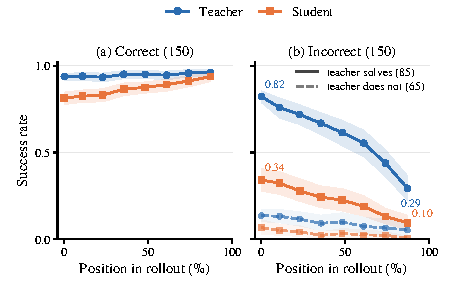
\includegraphics[width=\columnwidth]{figures/fig_failure_region.pdf}
% \caption{Expected accuracy of the teacher ($\Lambda^T$) and the student ($\Lambda^S$) from prefixes of the student on (a) correct and (b) incorrect rollouts.}
% \vspace{-0.25cm}
% \label{fig:failure-region}
% \end{figure}

% \noindent\textbf{The teacher retains recoverability on correct rollouts.}
% On correct rollouts (Figure~\ref{fig:failure-region}(a)), $\Lambda^T$ stays at or above 0.93 at every prefix, and $\Lambda^S$ rises from 0.81 to 0.94. The prefix of the student therefore does not by itself lower the accuracy of the teacher.

% \noindent\textbf{On incorrect rollouts, recoverability is lost to the prefix of the student or to the difficulty of the problem.}
% On problems that the teacher can solve (solid lines in Figure~\ref{fig:failure-region}(b)), $\Lambda^T$ is 0.82 at the empty prefix but falls to 0.29 along the incorrect rollout of the student, and $\Lambda^S$ falls from 0.34 to 0.10. This agrees with prior observations \citep{liu2026sfd, zhou2026early, li2026rethinking}. Together with the control in Figure~\ref{fig:failure-region}(a), it shows that the decline comes from what the student writes on an incorrect rollout rather than from the difficulty of the problem or the presence of a prefix. On problems that the teacher cannot solve (dashed lines), $\Lambda^T$ falls from 0.14 to 0.05, and recoverability is low mainly because the problems exceed the ability of the teacher. In both cases the premise of OPD fails, for different reasons: in the first case the student leads the teacher astray, and in the second case the teacher cannot solve the problem from the start.

% \noindent\textbf{More than half of the OPD supervision on incorrect rollouts falls on prefixes from which the teacher cannot recover.}
% We assign each token to the last cut before it and group the tokens by $\Lambda^T$ at that cut. Of the tokens of incorrect rollouts, 53\% come from prefixes with $\Lambda^T < 0.2$, and only 21\% come from prefixes with $\Lambda^T \geq 0.8$. Incorrect rollouts account for 61\% of the training tokens, so about one third of all training tokens come from prefixes from which the teacher itself rarely continues correctly. OPD still trains the student to imitate the teacher at these prefixes.

% \subsection{The Teacher Follows the Error but Still Recognizes It}
% \label{sec:critique-ability}

% We next ask why the teacher loses its recoverability and whether it also loses the ability to recognize errors. For the first question, we record the continuations of the teacher from each cut and check where its failed continuations end. For the second question, we split each truncated solution of the student into numbered paragraphs and ask the teacher to list its errors with the critique prompt of our method (Appendix~\ref{app:prompts}). In this test the teacher does not see the reference answer, so the test measures the ability that the teacher retains on its own, under a stricter condition than the critic of Section~\ref{sec:method}, which sees the reference answer. Qwen3-8B in thinking mode, which sees the reference answer, judges whether each listed error is real \tbd{agreement with human annotation}. We run both tests on the incorrect rollouts of problems that the teacher can solve, and Figure~\ref{fig:critique} shows the results.

% \begin{figure}[t]
% \centering
% 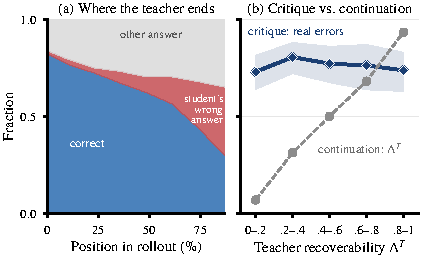
\includegraphics[width=\columnwidth]{figures/fig_critique.pdf}
% \caption{(a) Outcomes of the continuations of the teacher. (b) Fraction of the listed errors that are real and mean $\Lambda^T$ in each $\Lambda^T$ group. The band shows a 95\% bootstrap confidence interval.}
% \label{fig:critique}
% \end{figure}

% \noindent\textbf{When the teacher fails, it often follows the error of the student.}
% As the prefix grows longer (Figure~\ref{fig:critique}(a)), the fraction of correct continuations of the teacher falls from 0.82 to 0.30, and the fraction that ends with the original incorrect answer of the student rises from 1\% to 35\%, or from 8\% to 50\% of the failed continuations. The teacher almost never reaches this answer from the empty prefix, so these failures come from the rollout of the student. The teacher loses its recoverability not because it cannot solve the problem but because it accepts the errors in the prefix of the student.

% \noindent\textbf{The ability to recognize errors does not decline with recoverability.}
% Across the groups in Figure~\ref{fig:critique}(b), the mean $\Lambda^T$ rises from 0.07 to 0.93, whereas the fraction of listed errors that are real stays between 0.73 and 0.81. Even at prefixes with $\Lambda^T < 0.2$, this fraction is 73\%, which is comparable to the 74\% at prefixes with $\Lambda^T \geq 0.8$.

% Together, these results show that after the student errs, the teacher loses the ability to continue correctly but keeps the ability to critique. This suggests a path toward the goal of Section~\ref{sec:intro}. Existing methods treat the supervision at these prefixes as unreliable and avoid them by changing the training sequence. The teacher, however, still recognizes the errors at these prefixes, so the reliability of its supervision can be restored on the sequences of the student rather than avoided. Section~\ref{sec:method} builds CriticOPD on this ability and shows at the same cuts how the critique raises $\Lambda^T$ (Figure~\ref{fig:rewrite}).

\section{Measuring the Reliability of Teacher Supervision}
\label{sec:diagnosis}

This section measures the reliability of teacher supervision through recoverability and examines where and why OPD supervision becomes unreliable. Let $h_t=(x,y_{<t})$ denote a student-generated prefix, and let $r(y)\in\{0,1\}$ indicate whether a complete solution $y$ is correct. We define teacher recoverability as its expected accuracy when continuing from $h_t$,
$\Lambda^T(h_t)=\mathbb{E}_{y\sim\pi_T(\cdot\mid h_t)}[r(y)]$,
where $y$ denotes the completed solution. Student recoverability $\Lambda^S(h_t)$ is defined analogously using $\pi_\theta$.

$\Lambda^T$ measures the reliability of the teacher's continuation policy as a corrective target. Under the sampled reverse-KL objective, a student-sampled token $y_t$ receives the advantage
\setlength{\abovedisplayskip}{3pt}\setlength{\belowdisplayskip}{3pt}%
\begin{equation}
A_t = \log \pi_T(y_t \mid h_t)
    - \log \pi_\theta(y_t \mid h_t),
\label{eq:adv}
\end{equation}
which is positive when the teacher assigns $y_t$ a higher probability than the student. The OPD target at each prefix is therefore $\pi_T(\cdot\mid h_t)$. A student that perfectly imitates the teacher from $h_t$ onward would achieve accuracy $\Lambda^T(h_t)$. Thus, low recoverability indicates that the teacher's continuation policy is an unreliable corrective target, even though individual tokens may still be useful.

We measure both quantities using a Qwen3-1.7B student after 80 steps of OPD, the Qwen3-4B-Instruct-2507 teacher, and DAPO-Math-17k problems. The student generates one rollout for each of 900 problems, from which we randomly select 150 correct and 150 incorrect rollouts. We cut each rollout at the empty prefix and the seven paragraph boundaries nearest to $1/8,\ldots,7/8$ of its length. From each cut, the teacher and student each generate 16 continuations to estimate $\Lambda^T$ and $\Lambda^S$.

To distinguish prefix effects from problem difficulty, we divide incorrect rollouts by the success rate of the teacher on the original problem, which is $\Lambda^T$ at the empty prefix estimated from $16$ continuations: 85 come from problems with high initial teacher success ($\Lambda^T \geq 0.5$; solid lines in Figure~\ref{fig:failure-region}(b)), and 65 from problems with low initial success (dashed lines). Appendix~\ref{app:diagnosis} gives details and repeats the analysis with Qwen3-0.6B.

\begin{figure}[t]
\centering
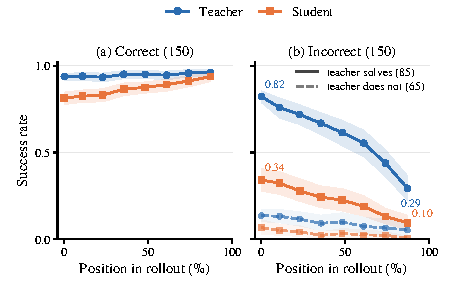
\includegraphics[width=\columnwidth,trim=0 7pt 0 0,clip]{figures/fig_failure_region.pdf}
\par\vspace{-4pt}
\caption{Teacher ($\Lambda^T$) and student ($\Lambda^S$) continuation accuracy along (a) correct and (b) incorrect rollouts.}
\label{fig:failure-region}
\vspace{6pt}
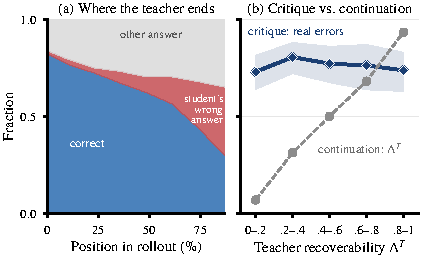
\includegraphics[width=\columnwidth]{figures/fig_critique.pdf}
\par\vspace{-4pt}
\caption{(a) Outcomes of teacher continuations. (b) Valid error-flag rate across teacher-recoverability bins.}
\label{fig:critique}
\end{figure}

\subsection{Recoverability Declines Along Incorrect Rollouts}
\label{sec:failure-region}

\noindent\textbf{The teacher retains recoverability on correct rollouts.}
On correct rollouts (Figure~\ref{fig:failure-region}(a)), $\Lambda^T$ stays at or above 0.93, while $\Lambda^S$ rises from 0.81 to 0.94. Thus, prefix growth alone does not explain the decline in teacher accuracy.

\noindent\textbf{Incorrect rollouts reduce teacher recoverability.}
On problems with high initial teacher success (solid lines in Figure~\ref{fig:failure-region}(b)), $\Lambda^T$ falls from 0.82 to 0.29, and $\Lambda^S$ from 0.34 to 0.10, consistent with prior observations \citep{liu2026sfd, zhou2026early, li2026rethinking}. Together with the control in Figure~\ref{fig:failure-region}(a), this suggests that the decline is associated with erroneous student prefixes rather than merely their length or problem difficulty. On problems with low initial teacher success (dashed lines), $\Lambda^T$ falls from 0.14 to 0.05, indicating that limited teacher capability is another source of unreliable supervision. Thus, OPD faces two difficulties: erroneous student prefixes can mislead an otherwise capable teacher, while some problems exceed the teacher's own ability.

\noindent\textbf{More than half of the tokens in incorrect rollouts receive supervision at low-recoverability prefixes.}
We assign each token to its preceding cut point and group tokens by $\Lambda^T$ at that cut. Among tokens in incorrect rollouts, 53\% correspond to prefixes with $\Lambda^T<0.2$, while only 21\% correspond to $\Lambda^T\geq0.8$. Since incorrect rollouts account for 61\% of training tokens, approximately one third of all training tokens receive supervision at prefixes from which the teacher rarely continues correctly.

\subsection{The Teacher Follows the Error but Still Recognizes It}
\label{sec:critique-ability}

We next examine why the teacher loses recoverability and whether it can still recognize errors. Both tests use the 85 incorrect rollouts from problems with high initial teacher success in Section~\ref{sec:failure-region}, without modifying the original trajectories.

First, we examine the final answers of teacher continuations from each cut. Second, we divide each nonempty prefix into numbered paragraphs and ask the teacher to identify its errors using our critique prompt (Appendix~\ref{app:prompts}). Unlike the critic in Section~\ref{sec:method}, the teacher receives no reference answer in this test. Qwen3-8B in thinking mode then judges each flagged error with access to the reference answer, labeling it as a new error, a propagated error, a restatement of an earlier error, or not an error. We count the first three categories as valid (Appendix~\ref{app:diagnosis}). This measures the validity of flagged errors rather than error-detection recall.

\noindent\textbf{The teacher often inherits the student's erroneous conclusions.}
As the prefix grows longer (Figure~\ref{fig:critique}(a)), the fraction of correct teacher continuations falls from 0.82 to 0.29, while the fraction ending with the student's incorrect answer rises from 1\% to 35\%, or from 8\% to 50\% of failed continuations. Since the teacher rarely produces this answer from the empty prefix, these results suggest that it often follows errors in the student prefix rather than failing solely because it cannot solve the original problem.

\noindent\textbf{Error recognition precision remains stable as recoverability declines.}
Across five bins of $\Lambda^T$ (Figure~\ref{fig:critique}(b)), mean recoverability ranges from 0.07 to 0.93, while the fraction of valid error flags remains between 73\% and 81\%. This fraction is 73\% at $\Lambda^T<0.2$ and 74\% at $\Lambda^T\geq0.8$. Thus, teacher continuation accuracy declines sharply, but critique precision remains stable.

